\documentclass[11pt]{article}
\usepackage[margin=1in]{geometry}

% Packages we need
\usepackage{amsmath}
\usepackage{amsfonts}
\usepackage{mathtools}
\usepackage{amsthm}
\usepackage{float}
\usepackage{graphicx}
\usepackage{listings}
\usepackage{color} %red, green, blue, yellow, cyan, magenta, black, white

% Header packages
\usepackage{fancyhdr}
\fancyhf{}
\pagestyle{fancy}

% Algorithms
\usepackage{algorithmic}
\usepackage{algorithm}

% Formatting document
\setcounter{secnumdepth}{0}
\setlength{\parindent}{0in}
\setlength{\parskip}{0.5em}

% MATLAB code
\definecolor{mygreen}{RGB}{28,172,0} % color values Red, Green, Blue
\definecolor{mylilas}{RGB}{170,55,241}

% Commands
\DeclarePairedDelimiter\ceil{\lceil}{\rceil}
\DeclarePairedDelimiter\floor{\lfloor}{\rfloor}
\newcommand{\ws}{\text{ }}
\newcommand{\e}[1]{\times 10^{#1}}

% Header
\lhead{\textsc{CS 5220 -- Project 1}} % TODO: enter title here
\rhead{\textsc{Eric Gao -- emg222\\Junteng Jia -- jj585}} % Authors
\setlength{\headheight}{0.5in}
\cfoot{\thepage}

% Title
\title{CS 5220 -- Project 1} %TODO: enter title here
\author{
  \begin{tabular}{l c l}
    Eric Gao & -- & emg222\\
    Junteng Jia & -- & jj585
  \end{tabular}\\
  \rule{\linewidth}{0.4pt}
}
\date{}


\begin{document}
    \thispagestyle{empty}
    \maketitle

    \section*{Results}
        \begin{figure}[H]
            \centering
            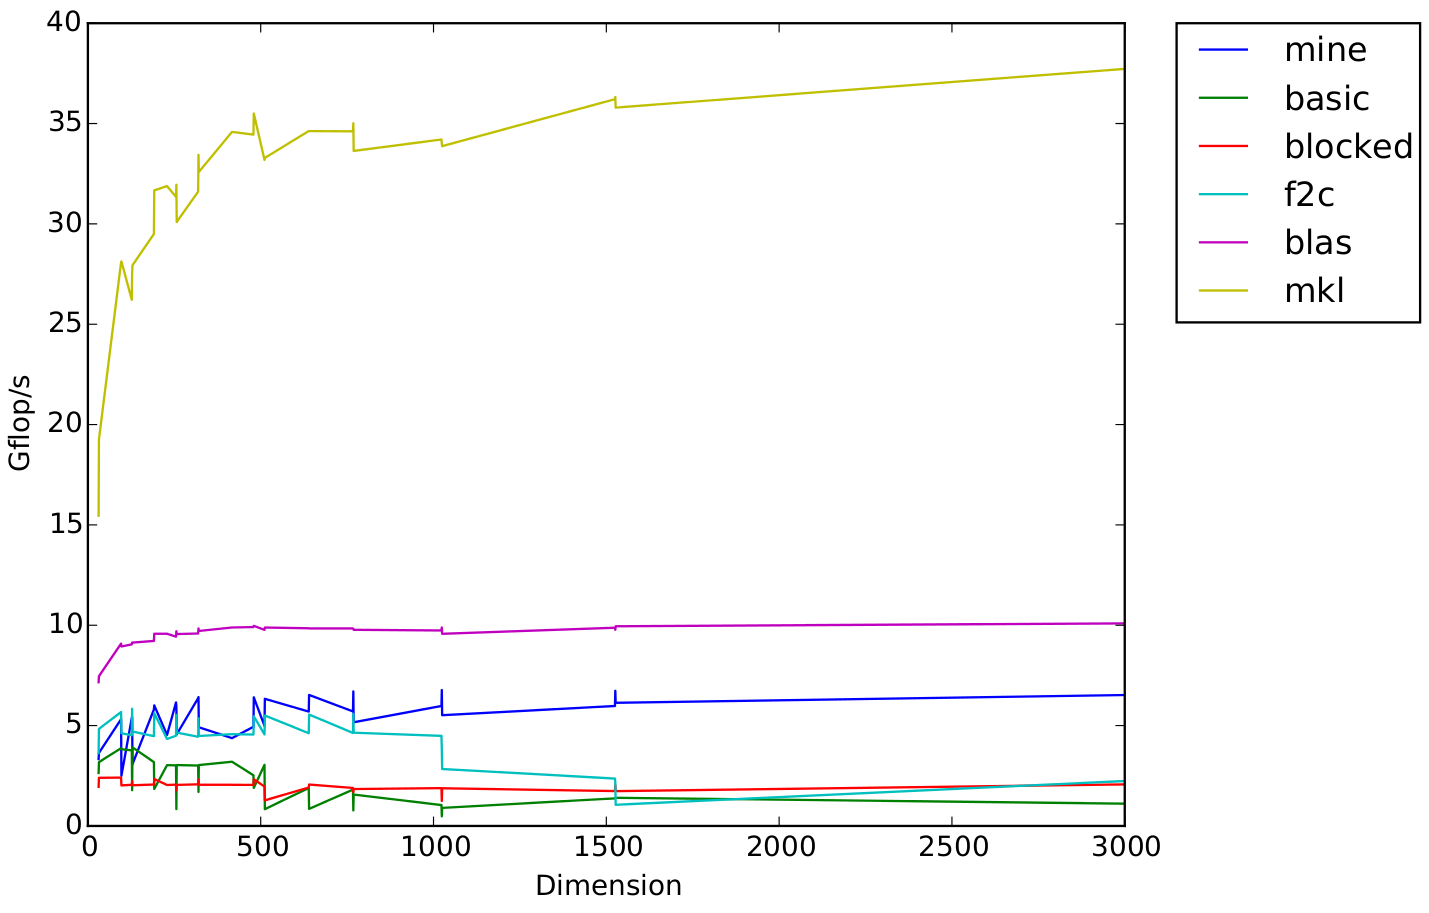
\includegraphics[width=6.5in]{timingvector32.png}
            \caption{Our results compared to other matrix multiplication implementation. Our code is comparable to the Fortran implementation for smaller matrices and runs faster for larger matrices.}
        \end{figure}

        We wrote this code from scratch and we beat Fortran. :)

    \pagebreak
    \section*{Our approach}
        We made four major improvements:
        \begin{enumerate}
            \item Block multiplication.
            \item Copy optimization.
            \item Data alignment.
            \item Vectorization.
        \end{enumerate}

        \subsection*{Block multiplication}
            We split the matrices into several blocks. We chose the blocks to be size 32, which means that each block takes up 8KB ($32^2 * 8$). This means we can fit all three blocks of the three matrices we care about into the L1 cache of the Phi processors since the L1 cache is 32KB. As a result, we can write a very fast kernel that allows us to take advantage of the fact that we know the size of the matrix and the fact that everything is in the L1 cache. This way, we can unroll our loops so we don't have to make unnecessary branching operations. We can then use this fast kernel to multiply blocks together so that we get the final result.


        \subsection*{Copy Optimization}
            We arranged the data so that within each block of $A$, the entries are row major and the blocks themselves are arranged in row major order. For $B$, the entries in the block are row major and the blocks themselve are arranged in column major order. We arrange them in this order so that we can have a stride of 1 for our kernel. This is to maximize spatial locality.

            Also, by doing this, we can handle fringe cases well. We make sure that matrices that we are multiplying have a leading dimension that is a multiple of our block size. We just add zeros on the edges to ensure this.

        \subsection*{Data alignment}
            We used the functions \texttt{\_mm\_malloc()} and \texttt{\_mm\_free()} so that we can guarantee that our matrices are aligned properly in memory. Specifically, we ensure that they are aligned to 64 bytes. We do this to ensure that we can take advantage of vector operations.

        \subsection*{Vectorization}
            We aligned our data to 64 bytes in memory and we multiply the blocks in our matrices in such an order so that we can take advantage of Vector FMAs. Specifically, we start with the (0, 0) element of a block in $A$. We multiply that by the first row of a block in $B$. We add that to the first row of a block in $C$. We then iterate across the 0th row of $A$ and iterate over the rows of the block in $B$. Then our outer loop iterates over the rows of $A$. This way, on our inner loop, we can take advantage of vector operations. When we compiled our code with the flags to show us whether we have vectorization, we obtained the following output:

            \begin{lstlisting}
LOOP BEGIN at dgemm_mine.c(121,13) inlined into dgemm_mine.c(199,17)
    remark #15388: vectorization support: reference C_row.286 has aligned access   [ dgemm_mine.c(124,17) ]
    remark #15388: vectorization support: reference C_row.286 has aligned access   [ dgemm_mine.c(124,17) ]
    remark #15388: vectorization support: reference B_row.288 has aligned access   [ dgemm_mine.c(124,17) ]
    remark #15399: vectorization support: unroll factor set to 8
    remark #15300: LOOP WAS VECTORIZED
    remark #15448: unmasked aligned unit stride loads: 2 
    remark #15449: unmasked aligned unit stride stores: 1 
    remark #15475: --- begin vector loop cost summary ---
    remark #15476: scalar loop cost: 13 
    remark #15477: vector loop cost: 4.000 
    remark #15478: estimated potential speedup: 3.220 
    remark #15479: lightweight vector operations: 6 
    remark #15480: medium-overhead vector operations: 1 
    remark #15488: --- end vector loop cost summary ---
LOOP END
            \end{lstlisting}


\end{document}